\subsection{Architecture and Application Characterization}
\begin{figure}
\begin{center}
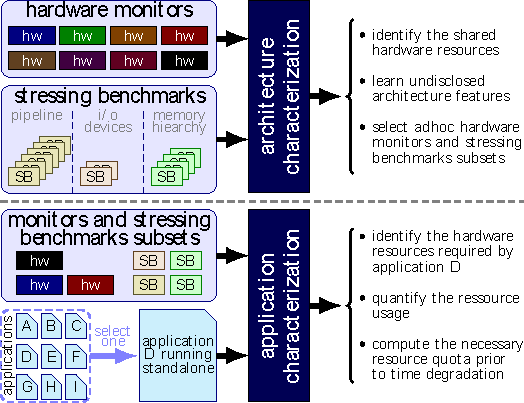
\includegraphics[width=0.7\textwidth]{\chapterdirectory/figure/micro_bench/co_running_apps_cots.pdf}
\end{center}
\caption{Strategy overview for \cite{Bin14} (Figure taken from the paper)}%
\label{fig:micro_bench:co_running_apps_cots}
\end{figure}

The approach presented in \cite{Bin14} can be seen as a follow up to the one of
\cite{10.1145/2086696.2086713}: the correlations between components that were
exposed are used to tailor the benchmarks performed on the application.  The
process is summarized in Figure~\ref{fig:micro_bench:co_running_apps_cots}.

When profiling the architecture, the objective is to characterize the hardware
itself, in order to identify shared hardware resources (including some that may
be missing from the architecture's documentation), determine their behavior when
in contention, potentially uncover unsuspected interactions between hardware
components, measure pertinent execution times and maximum bandwidths. To do so, the
approach starts with a comparison of each benchmark running in isolation and
running with other copies of itself running in parallel, as in the approach from
Section~\ref{sec:radojkovic} (the top-left diagonal in
Figure~\ref{fig:micro_bench:atom_stress}). In a second step, benchmarks
targeting different features are launched together. This provides information on
which parallel resource accesses affect one another. Here also, the approach is
similar to the one in Section~\ref{sec:radojkovic} (all cases other than the
top-left diagonal in Figure~\ref{fig:micro_bench:atom_stress}). Note that this
similarity with the previous section is to be expected, as both approaches make
similar assumptions on the availability of standard monitoring resources.  The
main difference being the use of hardware monitors other than the cycle counter
in \cite{Bin14}, where performance counters such as ``number of L1 hits'' are
also used in order to obtain a clearer understanding of the architecture, and
thus of the causes of the interference instead of just observing its effects.
This can be used to uncover relations between components despite not having
measured a change of slowdown factor upon their concurrent benchmarking.

Hardware monitors are counters that can be set to increase on the occurrence of
a given event, such as an access to the interconnect, a cache miss, a cache
eviction, and many other. The architecture's documentation generally provides a
list of events that can be monitored. These monitors can be reset, temporarily
frozen, or set to track another type of event during the execution of programs,
making them a very useful debugging and analysis tool.

\cite{Bin14} proposes using this information to limit the analysis made on
programs to what is truly necessary. Indeed, the architecture characterization
phase having already determined which combinations of benchmarks are redundant
for the analysis of interference between tasks, only a subset needs to be
employed to fully understand the impact of resource sharing on the
timing of the applications.

This subset of benchmark combinations is then used to analyze how much usage of
a particular resource is needed before an application slows down. In effect,
this indicates the minimal share of each resource needed for an application to
not suffer drastic worst case execution time slowdowns, and thus helps effective
scheduling of applications on a multi-core processor.

\begin{figure}[hbt!]
\begin{tabular}{cc}
\begin{subfigure}[t]{0.37\textwidth}
\lstinputlisting{\chapterdirectory/figure/micro_bench/paris_thesis_actual_general.txt}
\caption{Performance Counter Management}
\label{fig:micro_bench:co_running_apps_cots_algo_part_one}
\end{subfigure}
&
\begin{subfigure}[t]{0.47\textwidth}
\lstinputlisting{\chapterdirectory/figure/micro_bench/paris_thesis_general.txt}
\caption{Benchmark execution}
\label{fig:micro_bench:co_running_apps_cots_algo_part_deux}
\end{subfigure}
\end{tabular}
\caption{%
Benchmark algorithm used in \cite{Bin14} (extracted from \cite{Bin14Thesis})
}
\label{fig:micro_bench:co_running_apps_cots_algo}
\end{figure}

While \cite{Bin14} does not provide any code extracts, the algorithm can be
found in the associated thesis (\cite{Bin14Thesis}).
Figure~\ref{fig:micro_bench:co_running_apps_cots_algo} shows an overview of
algorithm used by \cite{Bin14}.
Figure~\ref{fig:micro_bench:co_running_apps_cots_algo_part_one} indicates how
the performance monitors are handled. The use of a loop to perform multiple
measures of the same experiment allow capture of the result's variability.
The benchmarked operations take the form shown in
Figure~\ref{fig:micro_bench:co_running_apps_cots_algo_part_deux}: it features an
unrolled loop (with \lstinline!UNROLLED! corresponding to the size of that inner
loop) within another loop, all performing the same operation (writing or
reading). The only reason for there to be an unrolled loop within the primary
loop is to reduce the amount of computations made during the iteration: the
combination of both loops simply makes the operations be performed across
the whole \lstinline!TABLESIZE! addresses. The \lstinline!STRIDE! parameter
corresponds to the gap between accesses, which is there to control the number of
times the same cache line is accessed. \cite{Bin14Thesis} indicates that the
use of the \lstinline!NOP! parameter is there to have idle time between
accesses: it corresponds to a varying number of \lstinline!nop! operations, and
can thus be used to see the effect of temporally spacing out the accesses.

The cache coherence identification part of this thesis
(Chapter~\ref{cha:identifying_cache_coherence}) uses an algorithm similar to the
one shown in Figure~\ref{fig:micro_bench:co_running_apps_cots_algo_part_one} to
observe the behavior of caches. In effect,
Chapter~\ref{cha:identifying_cache_coherence} is a specialized part of the
\textit{learn undisclosed architecture features} section of the
\textit{architecture characterization} process shown in
Figure~\ref{fig:micro_bench:co_running_apps_cots}. Instead of simply detecting
interaction It goes beyond the analysis
of simple interactions to really understand
\stopallthesefloats{}
